% Extensión estimada: unas 5 páginas, cinco subsecciones, cuatro tablas y una figura (ficha 4.4).
% Fuentes: ficha fichas/04-resultados-clasificacion/04-evaluaciones-complementarias.md; Codigo/outputs/results/
% hiba_por_modalidad.json y *_les_cwnone_hiba_predictions_hiba.json; robustness/robustness_summary.json;
% lesion_split_report.json (calibracion) y calibration_les/calibration_summary.json;
% interpretability_les/interpretability_swin.png (título recortado); cost/cost_comparison_v2.json.
% El label del costo es sec:res_costo_clasificadores: sec:res_costo es del Capítulo 5.
\section{Evaluaciones complementarias de la clasificación}
\label{sec:res_complementarios}

El diagnóstico del \emph{pipeline} lo fija un clasificador supervisado, pero todos sus resultados hasta aquí se
midieron sobre la prueba de \emph{HAM10000}, que comparte población, equipo de captura y forma de etiquetar con el
entrenamiento. Las cinco evaluaciones de la Sección~\ref{sec:met_complementarios} cambian esas condiciones o examinan
otros aspectos del clasificador: otra población, imágenes degradadas, la confianza de sus probabilidades, la región en
que se apoya y su costo. Salvo en el costo, que incluye los cuatro modelos, se usan Swin-Tiny y ConvNeXt-Tiny con la
semilla 42.

\subsection{Generalización a otra población}
\label{sec:res_hiba}

La primera evaluación lleva los dos clasificadores, sin ningún ajuste, a las 1\,616 imágenes de \emph{HIBA}. Como
muestra la Tabla~\ref{tab:res_hiba}, la sensibilidad macro de Swin-Tiny baja de 0.716 en la prueba de \emph{HAM10000} a
0.424, y la de ConvNeXt-Tiny, de 0.694 a 0.447. La caída es mayor en las fotografías clínicas, donde los dos quedan
por debajo de 0.27, pero también aparece en las imágenes dermatoscópicas, la misma modalidad del entrenamiento, con
0.494 y 0.519.

\begin{table}[H]
    \centering
    \caption{Sensibilidad macro en la prueba de \emph{HAM10000} y en \emph{HIBA}, por modalidad.}
    \label{tab:res_hiba}
    \small
    \setlength{\tabcolsep}{4pt}
    \begin{tabularx}{\textwidth}{@{}>{\raggedright\arraybackslash}X
        >{\centering\arraybackslash}p{2.3cm}>{\centering\arraybackslash}p{1.9cm}
        >{\centering\arraybackslash}p{2.9cm}>{\centering\arraybackslash}p{1.9cm}@{}}
        \toprule
        & & \multicolumn{3}{c}{\textbf{\emph{HIBA}}} \\
        \cmidrule(l){3-5}
        \textbf{Modelo} & \textbf{\emph{HAM10000}} & \textbf{Total} & \textbf{Dermatoscópicas} & \textbf{Clínicas} \\
        \midrule
        Imágenes & 1\,503 & 1\,616 & 1\,270 & 346 \\
        \midrule
        Swin-Tiny & 0.716 & 0.424 & 0.494 & 0.236 \\
        ConvNeXt-Tiny & 0.694 & 0.447 & 0.519 & 0.263 \\
        \bottomrule
    \end{tabularx}
\end{table}

La sensibilidad por clase muestra dónde se concentra esa caída. \gls{nv} se sostiene, con 0.930 en Swin-Tiny y 0.922
en ConvNeXt-Tiny, mientras que \gls{akiec} cae a 0.113 y 0.077. En esta clase influye el mapeo de diagnósticos de la
Sección~\ref{sec:met_hiba}, que lleva el carcinoma escamoso a \gls{akiec}: 158 de las 221 imágenes de esa clase en
\emph{HIBA} son carcinomas escamosos, un ruido que no puede separarse del cambio de población. Las demás clases, sin embargo, también bajan: \gls{mel} queda en 0.455 y 0.435, y \gls{bcc}, en 0.309 y
0.385. Por lo tanto, el desempeño medido en \emph{HAM10000} no se traslada a esta población, aun dentro de la misma
modalidad. Ninguno de los trabajos revisados en la Sección~\ref{sec:estado_arte_diagnostico} evalúa sus modelos en
población de América Latina, de modo que no hay una referencia con la que comparar esta caída.

\subsection{Robustez a perturbaciones de la imagen}
\label{sec:res_robustez}

Sin cambiar de población, la segunda evaluación degrada las imágenes de la prueba. La Tabla~\ref{tab:res_robustez}
muestra la caída relativa de la sensibilidad macro (Ecuación~\ref{eq:marco_robustez}) en el primero, el tercero y el
quinto nivel de cada perturbación. Como se mide con una sola vista y sin \gls{tta}, la base es algo menor que la de la
Tabla~\ref{tab:res_hiba}: 0.700 en Swin-Tiny y 0.680 en ConvNeXt-Tiny.

\begin{table}[H]
    \centering
    \caption{Caída relativa de la sensibilidad macro ante cuatro perturbaciones, por nivel de intensidad.}
    \label{tab:res_robustez}
    \small
    \setlength{\tabcolsep}{3pt}
    \begin{tabularx}{\textwidth}{@{}>{\raggedright\arraybackslash}X
        >{\centering\arraybackslash}p{1.1cm}>{\centering\arraybackslash}p{1.1cm}>{\centering\arraybackslash}p{1.1cm}
        >{\centering\arraybackslash}p{1.1cm}>{\centering\arraybackslash}p{1.1cm}>{\centering\arraybackslash}p{1.1cm}@{}}
        \toprule
        & \multicolumn{3}{c}{\textbf{Swin-Tiny}} & \multicolumn{3}{c}{\textbf{ConvNeXt-Tiny}} \\
        \cmidrule(lr){2-4}\cmidrule(l){5-7}
        \textbf{Perturbación (niveles 1, 3 y 5)} & \textbf{1} & \textbf{3} & \textbf{5} & \textbf{1} & \textbf{3}
            & \textbf{5} \\
        \midrule
        Compresión JPEG (calidad 70, 30 y 5) & 0.081 & 0.176 & 0.748 & 0.065 & 0.217 & 0.769 \\
        Ruido gaussiano (desvío 8, 32 y 64) & 0.184 & 0.685 & 0.796 & 0.244 & 0.725 & 0.790 \\
        Desenfoque (radio 1, 3 y 6) & 0.102 & 0.592 & 0.713 & 0.108 & 0.284 & 0.599 \\
        Resolución (0.75, 0.35 y 0.15) & 0.046 & 0.258 & 0.644 & 0.044 & 0.094 & 0.374 \\
        \bottomrule
    \end{tabularx}
\end{table}

En el primer nivel, la compresión, el desenfoque y la reducción de resolución quitan entre el 4\,\% y el 11\,\% de la
sensibilidad macro. El ruido gaussiano, en cambio, es la perturbación más dañina: con un desvío de 8 sobre 255 ya
quita el 18\,\% en Swin-Tiny y el 24\,\% en ConvNeXt-Tiny, y en el quinto nivel los dos modelos quedan en 1/7, es decir,
en el nivel del azar. Entre los dos modelos, ConvNeXt-Tiny soporta mejor la reducción de resolución y el desenfoque
intensos, con caídas de 0.374 y 0.599 en el quinto nivel frente a 0.644 y 0.713 de Swin-Tiny, mientras que en la
compresión y el ruido se comportan de manera parecida. Estas perturbaciones reproducen solo una parte de la variación
real entre equipos (Sección~\ref{sec:marco_eval_robustez}), así que no reemplazan la evaluación en \emph{HIBA}.

\subsection{Calibración}
\label{sec:res_calibracion}

Además de acertar la clase, el clasificador entrega probabilidades que fijan el umbral de melanoma y que un clínico
leería como certeza, y la tercera evaluación mide cuánto se puede confiar en ellas. La Tabla~\ref{tab:res_calibracion}
reúne el \gls{ece} y el Brier de los dos modelos sin calibrar, con los dos ajustes posteriores y en la versión
entrenada con pesos por clase.

\begin{table}[H]
    \centering
    \caption{Calibración en la prueba de \emph{HAM10000} (semilla 42).}
    \label{tab:res_calibracion}
    \small
    \setlength{\tabcolsep}{4pt}
    \begin{tabularx}{\textwidth}{@{}>{\raggedright\arraybackslash}X
        >{\centering\arraybackslash}p{1.2cm}>{\centering\arraybackslash}p{1.2cm}>{\centering\arraybackslash}p{2.1cm}
        >{\centering\arraybackslash}p{1.2cm}>{\centering\arraybackslash}p{1.2cm}>{\centering\arraybackslash}p{2.1cm}@{}}
        \toprule
        & \multicolumn{3}{c}{\textbf{Swin-Tiny}} & \multicolumn{3}{c}{\textbf{ConvNeXt-Tiny}} \\
        \cmidrule(lr){2-4}\cmidrule(l){5-7}
        \textbf{Versión} & \textbf{ECE} & \textbf{Brier} & \textbf{Sensibilidad macro} & \textbf{ECE} & \textbf{Brier}
            & \textbf{Sensibilidad macro} \\
        \midrule
        Sin calibrar & 0.040 & 0.233 & 0.716 & 0.040 & 0.231 & 0.694 \\
        \emph{Temperature scaling} & 0.027 & 0.234 & 0.716 & 0.027 & 0.231 & 0.694 \\
        \emph{Vector scaling} & 0.014 & 0.216 & 0.675 & 0.033 & 0.226 & 0.687 \\
        \filasep
        Con pesos por clase & 0.376 & 0.609 & 0.770 & 0.211 & 0.636 & 0.742 \\
        \bottomrule
    \end{tabularx}
\end{table}

Sin calibrar, los dos modelos tienen un \gls{ece} de 0.040, y su confianza media, de 0.820 en Swin-Tiny y 0.809 en
ConvNeXt-Tiny, es algo menor que su exactitud, de 0.847 y 0.845. Es decir, los modelos son levemente
subconfiados, y por eso la temperatura que ajusta la validación es menor que uno (0.850 y 0.859) y vuelve más
extremas las probabilidades. Con ese ajuste, el \gls{ece} baja a 0.027 sin cambiar ninguna predicción. El \emph{vector scaling}, en
cambio, sí cambia las predicciones, porque ajusta un parámetro por clase: en Swin-Tiny baja el \gls{ece} a 0.014,
pero la sensibilidad macro cae de 0.716 a 0.675. Los pesos por clase, por último, desarman la calibración. Con ellos,
el \gls{ece} sube a 0.376 en Swin-Tiny y a 0.211 en ConvNeXt-Tiny, porque la confianza media baja a alrededor de 0.4
mientras que la exactitud es de 0.775 y 0.599. En consecuencia, las probabilidades de los modelos sin pesos
pueden usarse casi sin corrección, y las de los modelos con pesos no deben leerse como certezas.

\subsection{Interpretabilidad}
\label{sec:res_interpretabilidad}

La cuarta evaluación examina en qué parte de la imagen se apoya Swin-Tiny para decidir. La
Figura~\ref{fig:res_gradcam} muestra el mapa de Grad-CAM de la primera imagen de cada clase en la prueba. En las cinco
imágenes que el modelo clasifica bien (\gls{bkl}, \gls{df}, \gls{mel}, \gls{nv} y \gls{akiec}), la activación se
concentra sobre la lesión. De los dos errores, el \gls{bcc} clasificado como \gls{mel} también activa la lesión, lo
que sugiere una confusión entre lesiones pigmentadas y no una decisión tomada sobre el fondo. El \gls{vasc}
clasificado como \gls{nv}, en cambio, tiene una activación difusa sobre la piel que rodea la lesión. Como se trata de
siete imágenes, la inspección muestra que el modelo puede apoyarse en la lesión, pero no mide con qué frecuencia lo
hace ni prueba un razonamiento clínico (Sección~\ref{sec:met_interpretabilidad}).

\begin{figure}[H]
    \centering
    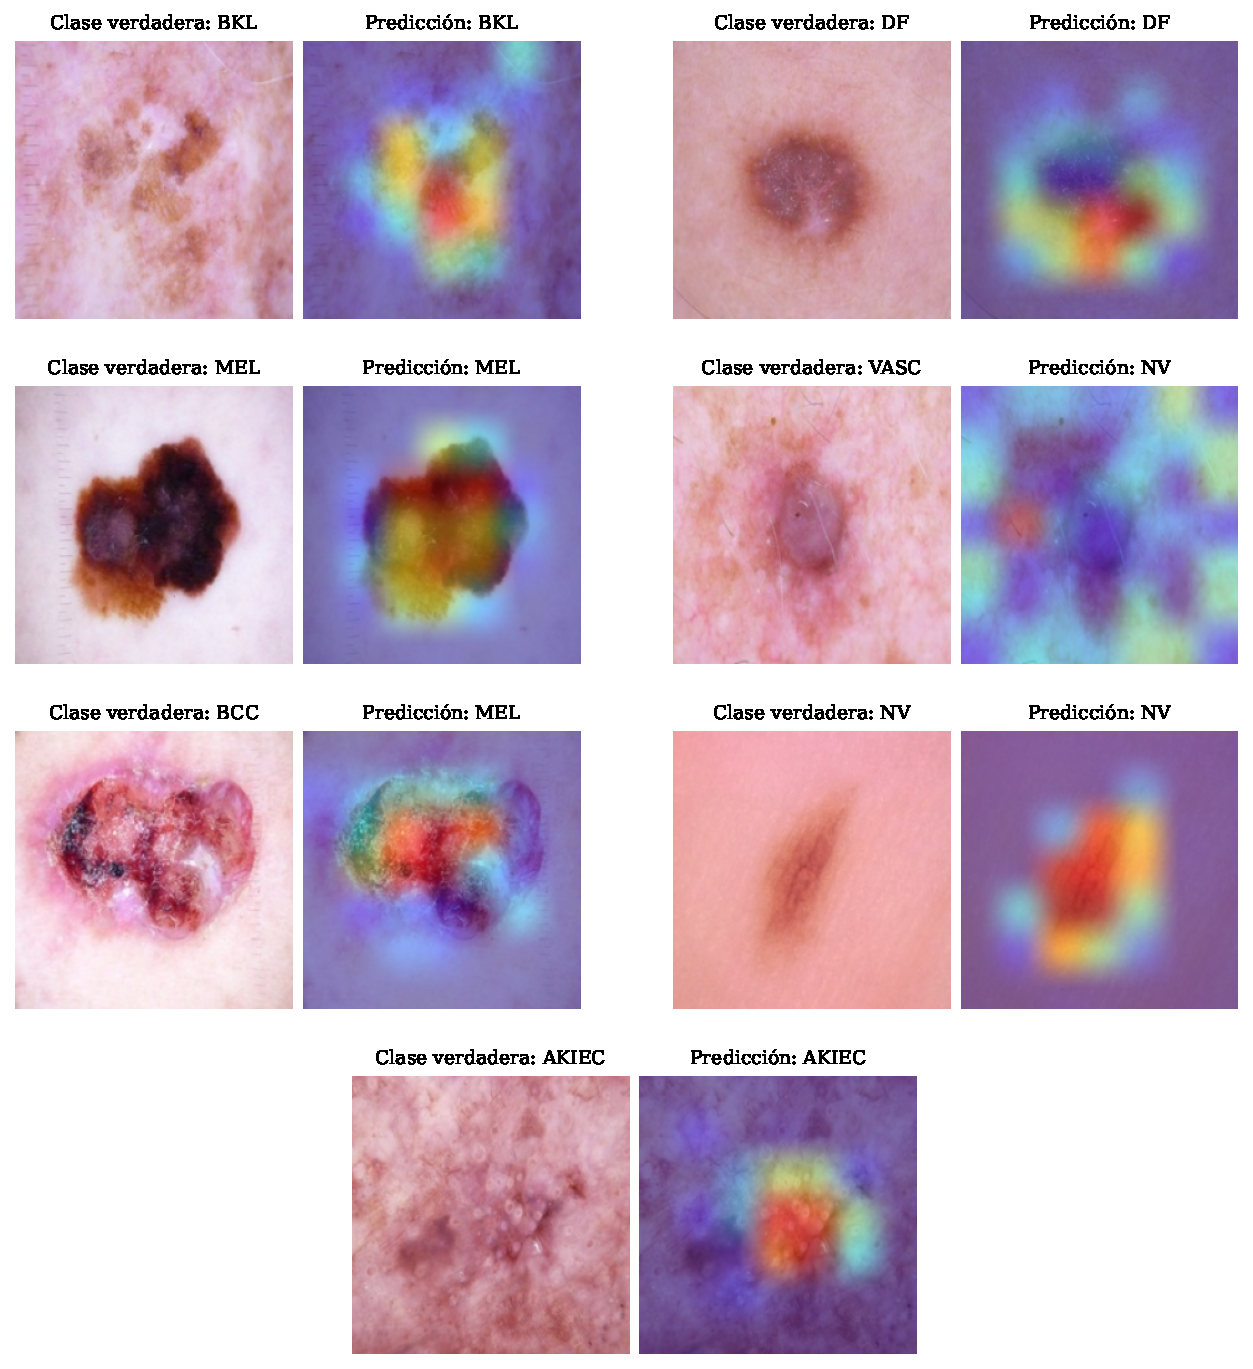
\includegraphics[width=0.9\textwidth]{Figures/Capitulos/04-Resultados-Clasificacion/gradcam-swin.pdf}
    \caption{Grad-CAM de Swin-Tiny sobre la primera imagen de prueba de cada clase.}
    \label{fig:res_gradcam}
\end{figure}

\subsection{Costo computacional de los clasificadores}
\label{sec:res_costo_clasificadores}

La última evaluación estima el costo de ejecutar los clasificadores en la RTX 4070 de la
Sección~\ref{sec:met_entorno}, con la misma precisión bf16 que la evaluación. Como muestra la
Tabla~\ref{tab:res_costo_clasificadores}, los cuatro modelos clasifican una imagen en 20~ms o menos, y la memoria
máxima que ocupan en la GPU, con lotes de 32 imágenes, no llega a 0.7~GB. Swin-Tiny, por ejemplo, tarda 11.1~ms por
imagen y procesa unas 1\,350 imágenes por segundo en lotes de 32, de modo que clasifica la prueba completa en poco
más de un segundo. Además, la cantidad de parámetros no ordena el tiempo de inferencia: DenseNet121, el modelo más
chico, es el más lento con una imagen por vez. Estos tiempos corresponden a una sola vista, y el \gls{tta} de la
Sección~\ref{sec:met_supervisados_receta}, que suma la imagen reflejada, requiere dos pasadas por imagen. Aun así, el
costo de los clasificadores queda muy por debajo del límite de una GPU de consumo que fija la
Sección~\ref{sec:met_tareas}.

\begin{table}[H]
    \centering
    \caption{Costo de inferencia de los clasificadores en una RTX 4070 (bf16, una vista por imagen).}
    \label{tab:res_costo_clasificadores}
    \small
    \setlength{\tabcolsep}{3pt}
    \begin{tabularx}{\textwidth}{@{}>{\raggedright\arraybackslash}X
        >{\centering\arraybackslash}p{1.9cm}>{\centering\arraybackslash}p{2.0cm}>{\centering\arraybackslash}p{2.0cm}
        >{\centering\arraybackslash}p{1.9cm}>{\centering\arraybackslash}p{2.0cm}@{}}
        \toprule
        & & \multicolumn{2}{c}{\textbf{Memoria máxima (GB)}} & & \\
        \cmidrule(lr){3-4}
        \textbf{Modelo} & \textbf{Parámetros (millones)} & \textbf{Una imagen} & \textbf{Lote de 32}
            & \textbf{Tiempo por imagen (ms)} & \textbf{Imágenes por segundo} \\
        \midrule
        Swin-Tiny & 27.52 & 0.180 & 0.522 & 11.05 & 1\,353.3 \\
        ConvNeXt-Tiny & 27.83 & 0.179 & 0.407 & 4.99 & 1\,738.5 \\
        ViT-B/16 & 85.80 & 0.511 & 0.678 & 5.72 & 903.5 \\
        DenseNet121 & 6.96 & 0.052 & 0.216 & 19.89 & 1\,700.3 \\
        \bottomrule
    \end{tabularx}
\end{table}

Con estas cinco evaluaciones, el clasificador queda caracterizado también fuera de las condiciones de su
entrenamiento: pierde buena parte de su desempeño en otra población, es sensible al ruido de la imagen, entrega
probabilidades bien calibradas cuando se entrena sin pesos y clasifica una imagen en 20~ms o menos, con menos de
0.7~GB de memoria de la GPU. La sección siguiente reúne lo que estos resultados y los de las secciones anteriores responden.
